\chapter{Estudo de Caso}
Este capítulo apresenta o estudo de caso conduzido com professores de \textit{introdução à programação} com o objetivo de investigar a viabilidade, utilidade prática e os desafios associados ao uso de templates multicamadas proposto neste trabalho. A pesquisa adota uma abordagem integrada à pesquisa-ação, com uso de métodos mistos (quantitativos e qualitativos). O estudo foi conduzido e estruturado para oferecer evidências que respondem às três questões de pesquisa (QP1, QP2 e QP3) conforme as diretrizes metodológicas recomendadas pela \gls{ceie} para estudos de caso.

\section{Objetivo do Estudo}
O objetivo deste estudo de caso é investigar a aplicabilidade da geração automática de questões utilizando templates multicamadas no contexto do ensino de programação, com base na experiência de professores na construção desses templates, e em suas percepções sobre a utilidade e os desafios da abordagem. Para isso, são apresentados a abordagem utilizada,  os procedimentos envolvidos e as métricas adotadas que fundamentam a coleta e análise dos dados que serão discutidos nas seções seguintes.
Embora não tenha sido possível aplicar o feedback automatizado aos participantes devido ao tempo limitado para o desenvolvimento deste estudo, a literatura  indica que este recurso tem potencial significativo para contribuir no aprendizado, como evidenciado por trabalhos como o de \parencite{vanpraet2024} e \parencite{fung2024} indicam que a incorporação de feedback automatizado se utilizado corretamente pode aumentar de forma significativa o desempenho dos estudantes.

\section{Metodologia do Estudo de Caso}

Este estudo adotou uma abordagem mista que combina técnicas quantitativas e qualitativas dentro de um ciclo de pesquisa. A opção por integrar essas abordagens decorreu de duas necessidades complementares: mensurar de forma objetiva, o tempo gasto, o número de questões produzidas e a taxa de reaproveitamento dos \textit{templates}, ao mesmo tempo em que se investigavam as percepções, dificuldades e sugestões dos professores.


\subsection{Perfil dos Professores}
Para garantir que os resultados reflitam um panorama representativo dos professores de Introdução a programação, foi definido dois critérios de inclusão e coleta de informação para cada professor com base nos seguintes aspectos: 

\begin{itemize}
    \item \textbf{Experiência recente}: lecionam ou lecionaram disciplinas introdutórias de programação em pelo menos 2 semestres nos cinco anos anteriores ao estudo.
    \item \textbf{Disponibilidade}: Compromisso para criar e avaliar templates e responder o questionário.
\end{itemize}

As Figuras \ref{fig:nivel-escolaridade}, \ref{fig:anos-docencia} e \ref{fig:linguagens-ensinadas} apresentam respectivamente, a distribuição dos participantes em relação ao nível de escolaridade, aos anos de experiência docente e às linguagens de programação ensinadas.

\begin{figure}[ht]
	\centering
	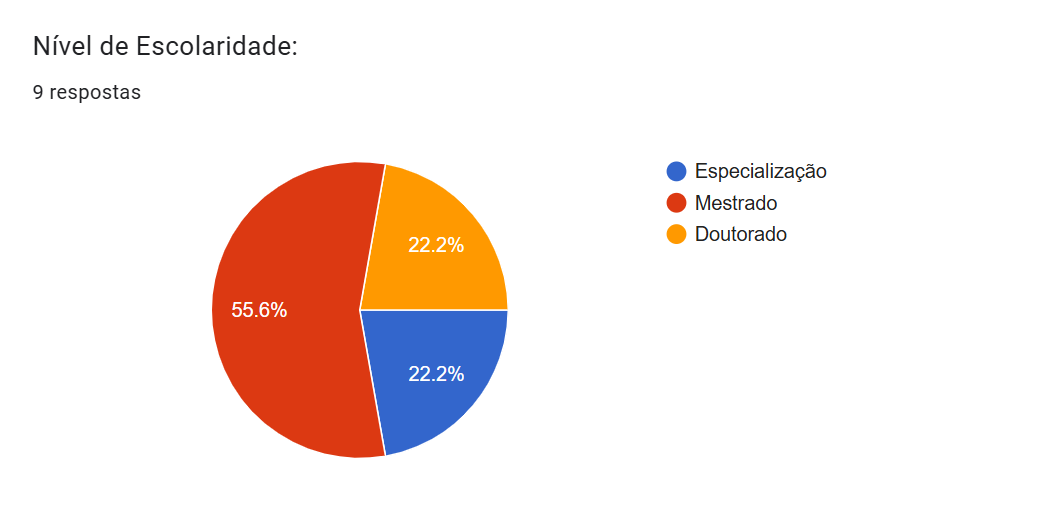
\includegraphics[width=16cm]{./imagens/capitulo8/1-escolaridade}
	\caption{Perfil Profissional 1 (Elaboração própria, 2025) }
	\label{fig:nivel-escolaridade}
\end{figure}
\begin{figure}[ht]
	\centering
	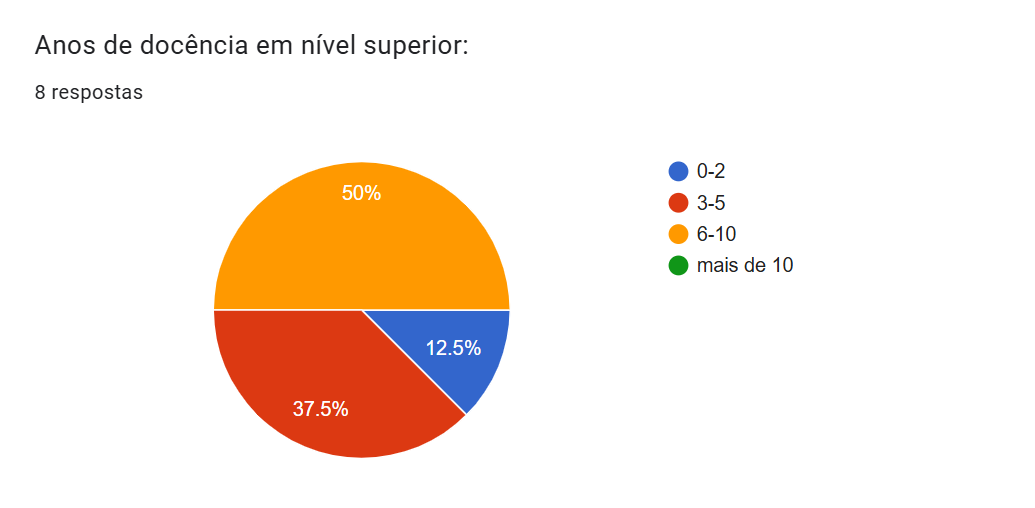
\includegraphics[width=16cm]{./imagens/capitulo8/2-anos-docencia}
	\caption{Perfil Profissional 2 (Elaboração própria, 2025) }
	\label{fig:anos-docencia}
\end{figure}
\begin{figure}[ht]
	\centering
	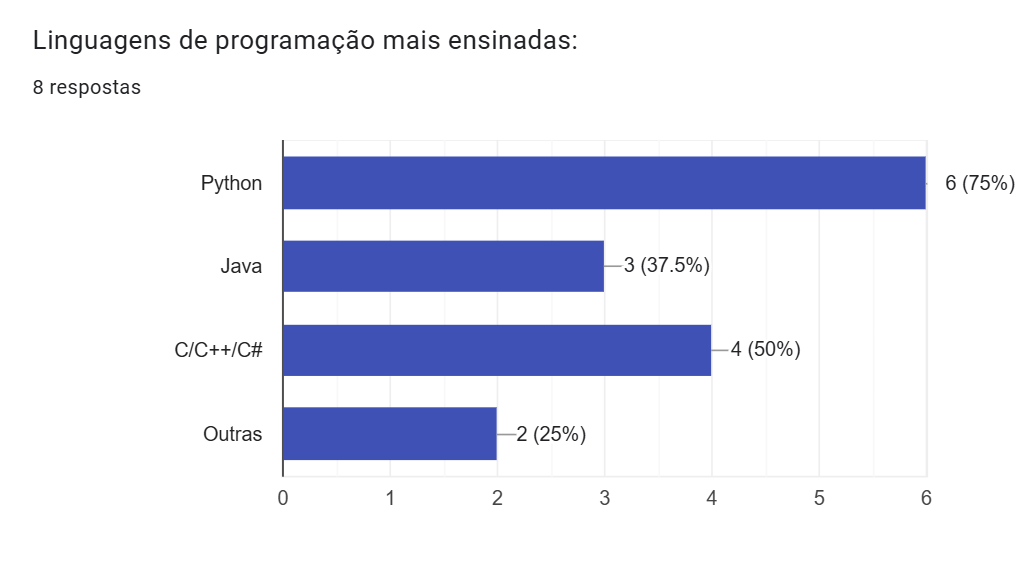
\includegraphics[width=16cm]{./imagens/capitulo8/2-linguagens-ensinadas}
	\caption{Perfil Profissional 3 (Elaboração própria, 2025) }
	\label{fig:linguagens-ensinadas}
\end{figure}

 
\subsection{Variáveis levantadas pelo questionário}
O formulário (ver Apêndice 1) foi dividido em 4 blocos, cada um mapeando uma das questões de pesquisa:

\begin{table}[H]
    \centering
    \begin{tabular}{|p{4cm}|p{5.4cm}|p{6cm}|}
        \hline
        \textbf{Bloco} & \textbf{Variáveis coletadas} & \textbf{Objetivo} \\ \hline
        Perfil profissional & Titulação, anos de docência, linguagens mais ensinadas. & Relacionar experiência ao \textbf{tempo médio} de criação de templates. \\ \hline
        Prática com templates & Tempo gasto, número de questões geradas, taxa de reaproveitamento. & Medir \textbf{viabilidade} e \textbf{utilidade} operacional. \\ \hline
        Percepções e desafios & Dificuldades encontradas, contribuição percebida, preferências de uso. & Identificar \textbf{barreiras} técnicas e pedagógicas. \\ \hline
        Adaptação de questões existentes & Grau de facilidade em converter questões próprias para o formato multicamada. & Verificar \textbf{capacidade de transformação} sem suporte externo. \\ \hline
    \end{tabular}
    \caption{Estrutura do questionário (Elaboração própria, 2025)}
    \label{tab:questionario-objetivos}
\end{table}

\subsection*{Etapas do Estudo}

O processo metodológico foi dividido em cinco etapas com a intenção de captar as percepções subjetivas dos professores:

\begin{enumerate}
    \item \textbf{Apresentação da proposta}: Foi exibido um vídeo curto dividido em três blocos (direcionamento, questões base e estrutura do modelo) com explicações sobre os fundamentos da geração automática de questões usando templates multicamadas, além de orientações de uso e exemplos práticos. O objetivo foi garantir a compreensão do assunto por parte dos professores.

    \item \textbf{Criação de templates pelos professores}: Após a apresentação do modelo, os professores elaboraram templates utilizando uma estrutura previamente definida. A orientação fornecida foi dividida em três tópicos principais:
    \begin{itemize}
        \item \textbf{Direcionamento}: Fundamentos e exemplos com perguntas-chave para ajudar na formulação do enunciado e identificação dos elementos variáveis.
        \item \textbf{Questões base}: Orientações para identificar os aspectos fundamentais do problema a ser transformado em questão.
        \item \textbf{Estrutura modelo}: Guia de construção do template, indicando como organizar o enunciado, variáveis e condições.
    \end{itemize}
    
    Os professores tiveram a disposição ferramentas de apoio, como uma estrutura básica do template e o \gls{chatgpt}, para auxiliar na criação e sugestão de variações e contextos. Esse suporte teve como objetivo facilitar a construção dos templates, ampliar as possibilidades de formulação.
\end{enumerate}


\subsection{Métricas e indicadores}

Para avaliar a utilidade prática dos templates, foram definidos três indicadores. Cada um deles foi escolhido por sua relevância direta às questões de pesquisa e por oferecer evidências sobre o esforço exigido, a produtividade e o potencial de reutilização dos templates gerados.
    \begin{itemize}
        \item \textbf{Tempo médio pra criação de um template} : intervalo em minutos, entre o inicio e o momento em que o professor considera o template pronto pra uso. Valores baixos indicam maior viabilidade operacional. A Figura \ref{fig:tempo-gasto}, mostra que a maioria dos professores avaliados levou em média 30 minutos para elaborar o template sugerido.
\begin{figure}[ht]
	\centering
	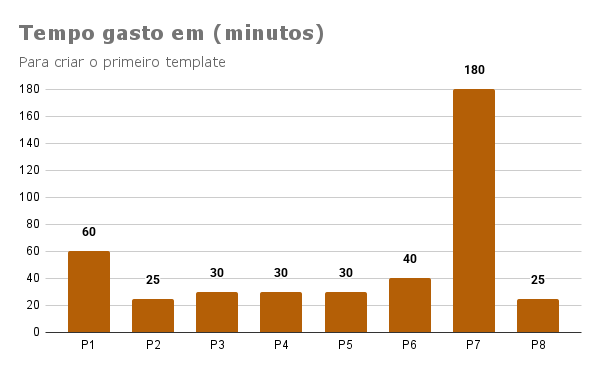
\includegraphics[width=14cm]{./imagens/capitulo8/tempo-gasto}
	\caption{Tempo médio de criação do primeiro template (Elaboração própria, 2025) }
	\label{fig:tempo-gasto}
\end{figure}
        \item \textbf{Numero de questões geradas por template} : quantidade total de instâncias de questões produzidas a partir de um único template, considerando as combinações válidas de variáveis, quanto maior o repertório de questões geradas maior o poder de generalização do template.
\begin{figure}[ht]
	\centering
	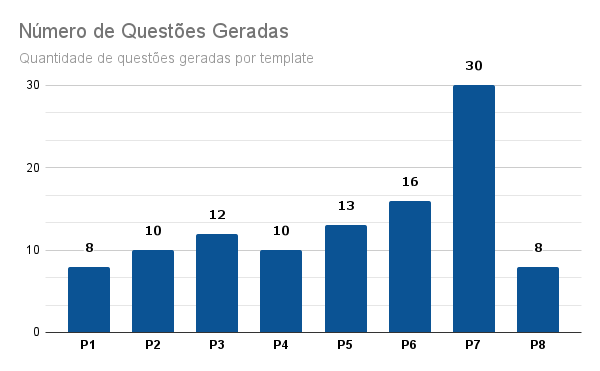
\includegraphics[width=14cm]{./imagens/capitulo8/questoes-geradas}
	\caption{Numero de questões geradas por template (Elaboração própria, 2025) }
	\label{fig:questoes-geradas}
\end{figure}
        \item  \textbf{Sucesso em converter a questão existente em template }: indica se foi possível ou não transformar uma questão existente em um template funcional, mantendo sua essência pedagógica, o questionário indicou que todos os participantes responderam "sim" para conversão de uma questão existente em template, com exceção de um. 
        \item \textbf{Dificuldades encontradas:} Após a construção do template proposto, a principal dificuldade relatada pelos participantes foi organizar adequadamente as ramificações entre as camadas, conforme ilustrado na Figura \ref{fig:dificuldades-encontradas}.  
    \end{itemize}


\begin{figure}[ht]
	\centering
	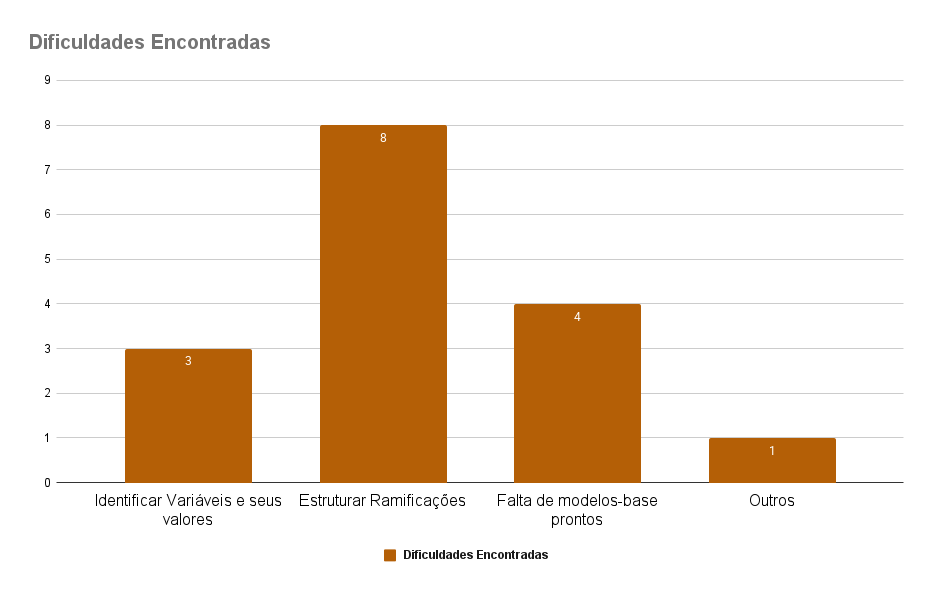
\includegraphics[width=14cm]{./imagens/capitulo8/dificuldades-encontradas}
	\caption{Dificuldades encontradas  (Elaboração própria, 2025) }
	\label{fig:dificuldades-encontradas}
\end{figure}



\section{Resultados Observados}

Para além dos indicadores objetivos foi aplicado um bloco de afirmações em escala \textit{Likert} (5 = \textit{Concordo totalmente} .... 1 = \textit{Discordo totalmente})  para entender como os professores enxergam a abordagem. A Tabela \ref{tab:dimensoes-likert} apresenta uma síntese dos resultados exibidos nas Figuras \ref{fig:preferencia-uso}, \ref{fig:intencao-uso} e \ref{fig:percepcao-utilidade}, agrupando-os em três dimensões principais.

\begin{table}[H]
    \centering
    \caption{Síntese comparativa das dimensões avaliadas na escala Likert (N = 8)}
    \label{tab:dimensoes-likert}
    \begin{tabular}{|p{0.15\textwidth} |p{0.40\textwidth} |p{0.35\textwidth}|}
        \hline
        \textbf{Dimensão} & \textbf{Principais evidências levantadas} & \textbf{Implicação para as QPs}\\ \hline
        Preferência de Uso &
             \textbf{Adaptação}: 7 de 8 dos professores \textit{concordam} ou \textit{concordam totalmente} que preferem adaptar modelos prontos. \newline%
             \textbf{Criação do zero}: 5 de 8 \textit{discordam} ou \textit{discordam totalmente} de criar tudo do zero.%
         &
        Reforça a \textbf{viabilidade operacional} do repositório-base (QP1) e o potencial de \textbf{reutilização}. \\ \hline
        Intenção de Uso &
            6 de 8 professores indicariam a ferramenta a outros professores. Mas o uso na disciplina dividiu opiniões (4 neutras e 4 negativas)%
        \ &
        Sinaliza \textbf{barreiras de adoção} que exigem suporte, necessita de uma adequação na abordagem. \\ \hline
        
        Percepção de Utilidade &
            Todos compreenderam a estrutura dos templates.\newline%
            Todos concordaram que o ChatGPT facilita muito as variações.\newline%
            4 de 8 professores julgaram a curva de aprendizagem longa.%
         &
        a curva de aprendizagem evidencia um \textbf{custo inicial} (QP3), precisa de muito esforço cognitivo para o entendimento conceitual. \\ \hline
    \end{tabular}
\end{table}



\begin{figure}[ht]
	\centering
	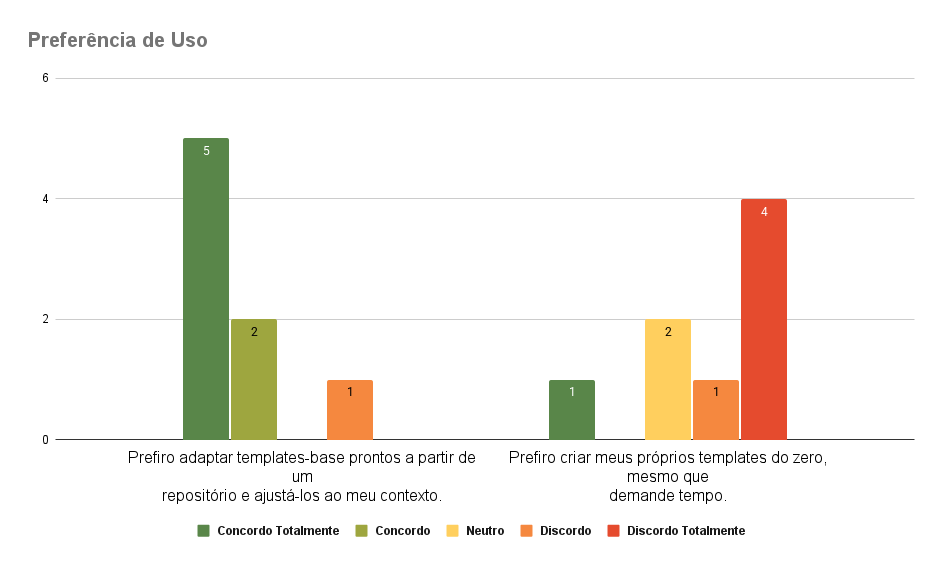
\includegraphics[width=16cm]{./imagens/capitulo8/preferencia-uso}
	\caption{Preferencia de uso  (Elaboração própria, 2025) }
	\label{fig:preferencia-uso}
\end{figure}


\begin{figure}[ht]
	\centering
	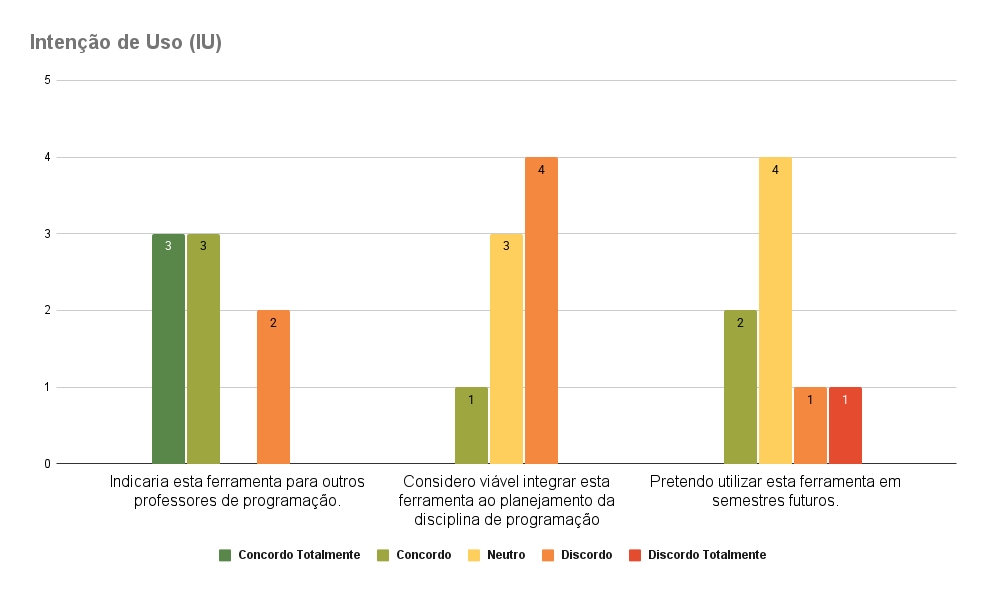
\includegraphics[width=16cm]{./imagens/capitulo8/intencao-uso}
	\caption{Intenção de uso  (Elaboração própria, 2025) }
	\label{fig:intencao-uso}
\end{figure}



\begin{figure}[ht]
	\centering
	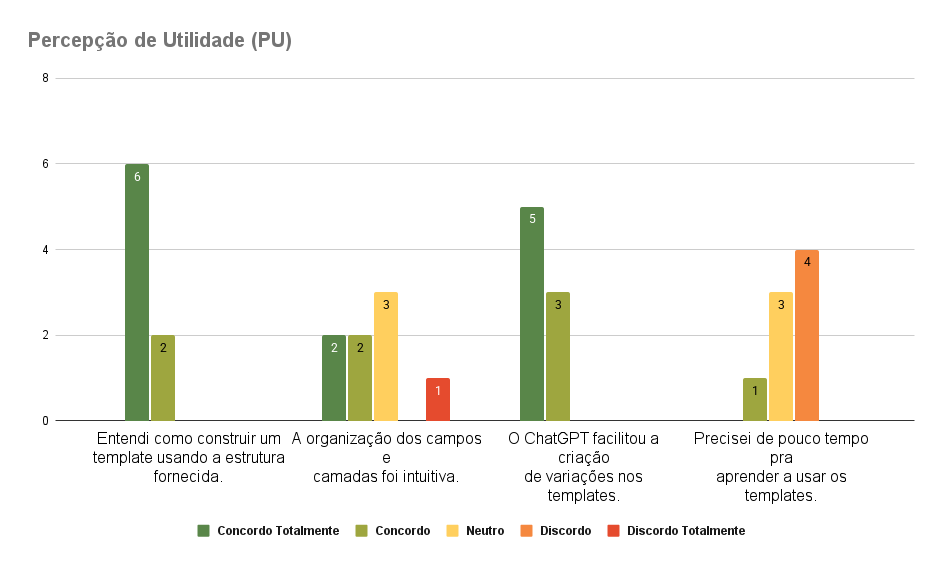
\includegraphics[width=16cm]{./imagens/capitulo8/percepcao-utilidade}
	\caption{Percepção de utilidade  (Elaboração própria, 2025) }
	\label{fig:percepcao-utilidade}
\end{figure}

	
\section{Relatos de respostas abertas}

As respostas abertas fornecidas pelos professores no questionário revelam  informações que complementam os dados apresentados anteriormente. De modo geral, muitos professores relataram que a maior dificuldade está no esforço mental em visualizar o funcionamento de um template multicamadas de forma textual. Essa limitação impacta diretamente a compreensão do fluxo lógico, a previsão de combinações corretas e a identificação de erros durante a elaboração. Muitos apontaram que, sem o apoio de ferramentas como o ChatGPT, a construção seria muito demorada e sujeito a erros.

Apesar das dificuldades, os relatos revelaram pontos positivos e sugestões importantes. Houve reconhecimento do potencial da abordagem para diversificar os exercícios e reduzir o retrabalho. Além disso os professores também apresentaram algumas sugestões de melhora conforme a tabela \ref{tab:relatos-abertos}.


\begin{table}[H]
\centering
\caption{Síntese dos relatos abertos (N~= 8)}
\label{tab:relatos-abertos}
\begin{tabular}{|p{0.24\textwidth} |p{0.28\textwidth} |p{0.32\textwidth}|}
\hline
\textbf{Categoria} & \textbf{Principais evidências} & \textbf{Necessidades/sugestões} \\ \hline
\textbf{Desafios cognitivos} & 
    “Exige muita abstração”; \newline
    “Difícil enxergar o template usando JSON”
& Visualização em camadas; exemplos visuais \\ \hline
\textbf{Curva de aprendizagem} & 
    “Curva de aprendizado é uma limitação”;\newline
     "Dependência do ChatGPT para começar"
 & Repositório de modelos-base; tutoriais passo a passo \\ \hline
\textbf{Manipulação de JSON} & 
    “Difícil manipular texto JSON” \newline
    "Erros de sintaxe e concordância"
 & Editor visual + validador automático \\ \hline
\textbf{Tempo de elaboração} & 
    “Tempo gasto em pensar no formato é alto” 
& Assistente de pré-visualização e depuração \\ \hline
\textbf{Benefícios percebidos} & 
    “A ideia é boa” \newline
    “ChatGPT facilitou muito”
 & Manter integração com IA; ampliar exemplos \\ \hline
\end{tabular}
\end{table}

A análise das respostas abertas revelou quatro principais obstáculos enfrentados pelos professores durante a abordagem que são : 

\begin{enumerate}
    \item \textbf{Visualização da lógica}: a ausência de uma representação gráfica torna difícil acompanhar onde cada variável é inserida e como as ramificações são formadas.
    \item \textbf{Falta de modelos-base}: Alguns professores sentiram dificuldade para iniciar a construção do template, devido a \emph{falta de modelos-base prontos}, essa foi a terceira dificuldade mais citada.
    \item \textbf{Sintaxe JSON}: erros simples (vírgulas, chaves) quebram o template inteiro; isso desestimula a edição manual.
    \item \textbf{Tempo e dependência de IA}: ainda que o ChatGPT acelere o processo, há receio de criar templates tendenciosos capazes de tornar as questões enviesadas.
\end{enumerate}

E com relação a sugestões de melhoria, quase todos os participantes apontaram de forma recorrente três aspectos principais:

\begin{enumerate}
\item \textbf{Interface gráfica baseada em blocos}:  que possibilite “arrastar e soltar” as camadas, condições e variáveis, para reduzir a necessidade de manipular o texto puro.
\item \textbf{Pré-visualizador dinâmico}: capaz de executar combinações em tempo real e verificar a coerência das questões geradas.
\item \textbf{Repositório de templates}: para servir como ponto de partida e material de apoio.
\end{enumerate}

\subsection{Limitações e Ameaças à Validade}
Apesar dos resultados encontrados, é essencial analisar cuidadosamente a validade do estudo. A seguir, são apresentados  três fontes principais de limitação que devem ser levadas em conta na interpretação dos dados:
\begin{itemize}
\item \textbf{Amostra restrita}: apenas oito professores participaram do estudo, o que pode limitar a generalização.
\item \textbf{Variabilidade de experiência}: diferenças no domínio técnico dos professores podem ter influenciado tanto o tempo de criação quanto a percepção de utilidade.
\item \textbf{Dependência de uma única ferramenta de IA}: os resultados podem ser diferentes com outros LLMs ou versões futuras do ChatGPT.
\end{itemize}



\subsection{Implicações para as Questões de Pesquisa}

O estudo de caso permitiu avaliar os pontos fortes e limitações do modelo proposto. As respostas do estudo de caso indicam que o modelo é útil em determinados cenários, mais também necessita de ajustes e aprimoramentos.
Essas evidências tem implicações diretas para as três questões de pesquisa definidas no início da dissertação que serão respondidas no próximo capitulo que são as considerações finais. Além disso, serão apontadas as direções para trabalhos futuros que possam superar as limitações identificadas neste estudo.